
\begin{figure}[t]
    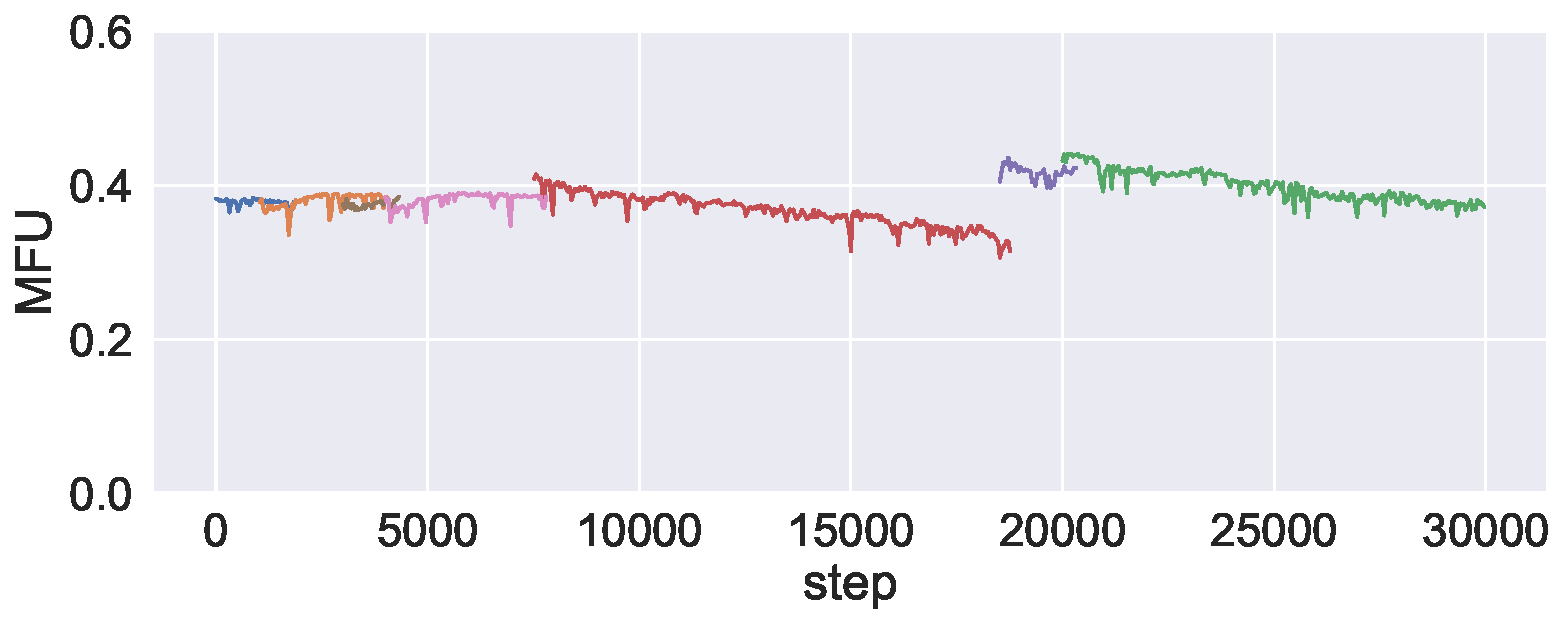
\includegraphics[width=0.46\textwidth]{figures/experience/mfu-straggler.pdf}
    \caption{Inconsistent MFU observed in large-scale training. Different colors denote distinct executions of the same training job.}
    \label{fig:mfu-straggler}
\end{figure}


\section{Training Troubleshooting}
\label{sec:monitor}

Although our robust training framework automatically discovers, pinpoints, and
resolves the majority of common faults, there remain certain hardware anomalies
that manifest probabilistically and cannot be found by machine self-checks. Some
anomalies may make the system appear to operate normally, yet significantly
degrades the training efficiency.
To address these nuanced cases, we have
implemented several custom monitoring and analysis tools designed to support
case-by-case anomaly detection.

\subsection{Performance Diagnosis with CUDA Event Monitor}



At the scale of tens of thousands of GPUs, we observe that, unlike in
smaller-scale experiments, different runs exhibit varying computational
efficiencies. Even with identical configurations , this inconsistency persist, as shown in Figure \ref{fig:mfu-straggler}. We also observed that the performance of training tasks is not consistent at this scale. The MFU for various training tasks gradually declines over time. While this leads us to suspect variations between individual machines, no evident variations are detected under single GPU GEMM micro-benchmarks. To diagnose those performance issues, we develop a performance analysis tool that records the execution
time of critical code segments on each machine rank during a run. In contrast to
previous tools such as the torch profiler or the Megatron-LM timer, our tool times
events based on the CUDA events method. This approach minimizes the need for
CUDA synchronization, thus preventing performance degradation, allowing us to
consistently run it in our production training jobs. This tool offers two
visualization modes and can analyze the collected data from different
perspectives.


\begin{figure}[t!]
    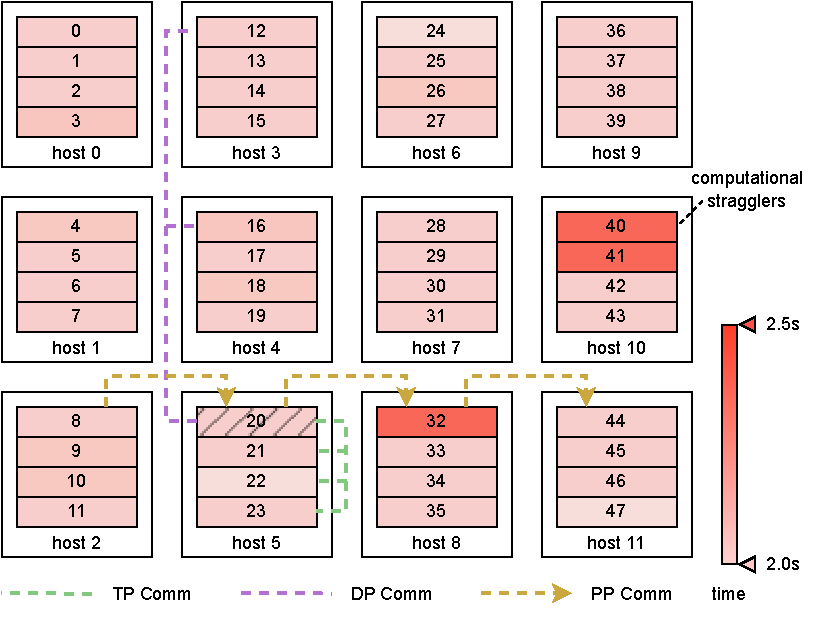
\includegraphics[width=0.45\textwidth]{figures/training-diagnosis/heatmap.pdf}
    \caption{Performance heat-map. The color denotes the running time of the code segments on a rank. The figure also shows the 3D visualization feature, where rank 20 has been selected and the dependency across different parallelism dimensions become visible.}
    \label{fig:heatmap}
\end{figure}

The first mode uses a heat map to show time consumption differences between
machines from various dimensions, depicted in Figure \ref{fig:heatmap}. We gather latency data of the computation
phase (forward and backward) across devices and average the latency across
steps. The aggregated data is visualized using a heat-map. The heat-map reveals
that a minor fraction of machines (approximately 0.5\%) exhibit substantially
slower performance during training, thereby hindering overall training progress.
The training efficiency is predominantly determined by the slowest machine's
performance (\ie, stragglers), leading to inconsistencies in training efficiency
across diverse runs, since machine scheduling within the cluster is stochastic.
After excluding these outlier machines, the peak MFU across runs becomes
consistent.

The other mode displays the event timeline on machines in a trace format from different distributed views (data parallelism, pipeline parallelism, tensor parallelism). Traditional profiler, such as PyTorch Profiler, is primarily designed for single-node activity analysis. This approach offers limited insight in distributed training scenarios where execution dependencies frequently span across multiple nodes. By aggregating the trace spans of various ranks onto a singular timeline, we gain a comprehensive perspective, revealing the overall execution order, pipeline bubbles, and synchronization characteristics among data parallel ranks. Figure \ref{fig:trace} displays how our distributed tracer visualizes the actual execution of pipeline parallelism, detailing the data dependencies between different pipeline stages through the consolidation of event data across a pipeline parallelism group.
%The resulting visualization bears a strong resemblance to trace files exported via PyTorch Profiler. 

Every piece of data from the CUDA event timer is stored in a remote analytical database, allowing for easy retrieval of details from any step event. While the timer data is wrote to a local file in a line-by-line format, a separate streamer process then synchronizes this log file with a Kafka queue in real-time. The analytical database remains updated by consuming data from this Kafka queue, enabling on-the-fly analysis without interrupting the training job. \revision{All the monitoring features are turned on during real production training and the overhead is negligible compared to the training time.}


\begin{figure*}
    \centering
    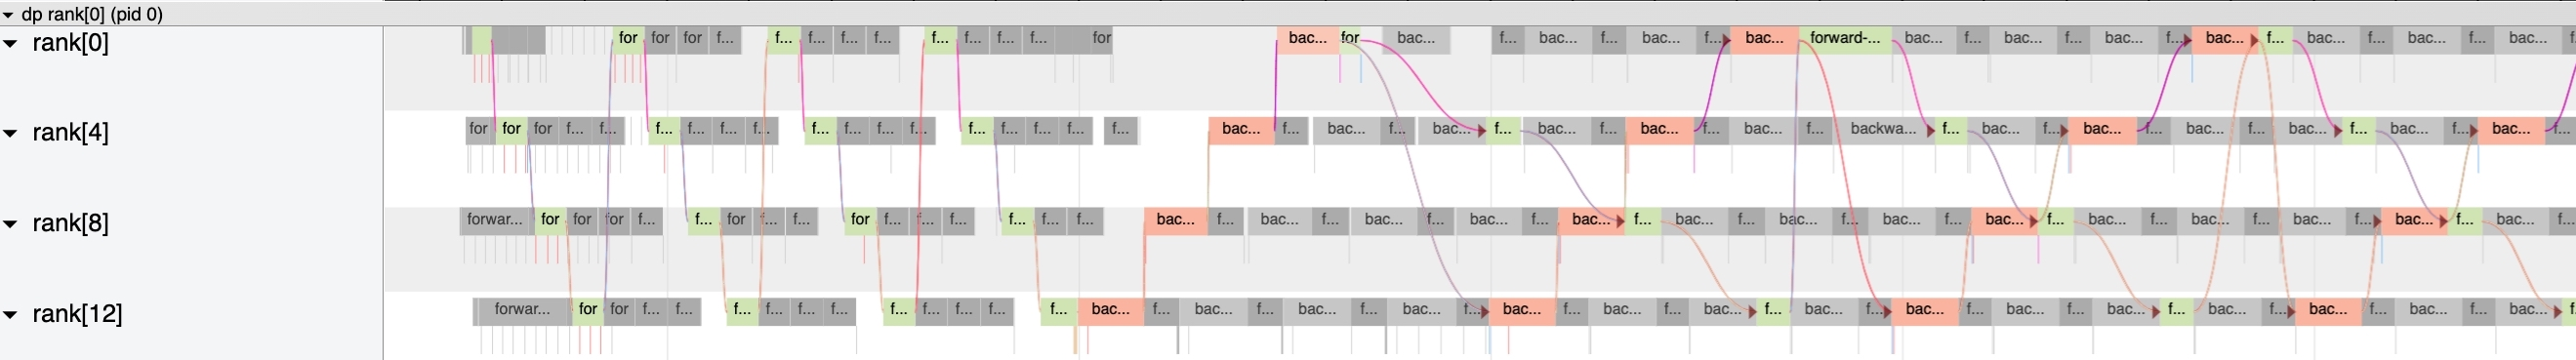
\includegraphics[width=0.95\textwidth]{figures/training-diagnosis/trace.jpeg}
    \caption{The trace shows events collected in a pipeline group on a unified timeline. Dependencies become visible when an event is selected.}
    \label{fig:trace}
\end{figure*}


\subsection{3D Parallel Training Visualization}
\label{sec:visualization}

With 3D parallelism and our optimization techniques (\S\ref{sec:train}), the landscape of data flow and task sequencing is
exceedingly intricate. Each GPU worker may be engaged in several synchronous
or asynchronous operations at the given moment, leading to complex
dependencies among them. This intricacy amplifies the challenges of fault
diagnosis: when a single GPU worker experiences a fault, the entire cluster of
nodes can stall in the NCCL communication operations, ultimately leading to a
system-wide timeout. Externally, this situation manifests as a generic blockage,
but the root cause of which is often buried under a deluge of timeout messages.
To rapidly pinpoint the problematic nodes, we let each GPU worker log its own
ongoing event upon communication timeout. These logs are then used to construct
a visual representation of data dependencies based on the logical topology in
the 3D parallel setting.

As Figure~\ref{fig:heatmap} shows, the cluster in 3D parallel training can
logically be split into three dimensions: tensor parallelism, pipeline
parallelism, and data parallelism. When we select a specific GPU worker, it
displays its position within the logical topology, the direction of data flow
and the different communication operations it involves. Importantly, in the
event of an error, the tool provides direct access to the worker's error
messages if any. This serves as a powerful tool for diagnosing training
anomalies, enabling quicker identification and resolution of faults.

Consider the aforementioned case when defective GPUs probabilistically cause blocking when executing NCCL communication operations. Such blocking can hang the entire machine, leading to cascading timeouts across other dependent nodes and ultimately resulting in the paralysis of the entire training process. To swiftly identify these faulty nodes, we utilize the 3D parallel training visualization tool. Nodes that timeout due to waiting for the faulty ones will log their ongoing operations upon exiting. In contrast, the nodes with the faulty GPUs are hung and do not log any such information. Therefore, by examining the logs and the data flow within the visualization, these problematic nodes can be easily pinpointed. Once identified, these nodes can be manually isolated and flagged for maintenance through the robust training framework, as described in \ref{sec:robust_training_workflow}.